\lstinputlisting[language=bash,basicstyle=\small]{python_codes/fieldstone_18/keywords}

\begin{center}
Code at \url{https://github.com/cedrict/fieldstone/tree/master/python_codes/fieldstone_18}
\end{center}

\par\noindent\rule{\textwidth}{0.4pt}
%%%%%%%%%%%%%%%%%%%%%%%%%%%%%%%%%%%%%%%%%%%%%%%%%%%%%%%%%%%%%%%%%%%%%%%%%%%%%%%%%%%%%%%%%%%%

\subsubsection*{Donea \& Huerta benchmark}
The details of the numerical setup are presented in Section \ref{mms1}.

Each element has $m_V=9$ vertices so in total $ndof_V\times m_V=18$ velocity dofs and 
$ndof_P*m_P=4$ pressure dofs. The total number of 
velocity dofs is therefore $NfemV=NV \times ndofV$ while the total number of
pressure dofs is $NfemP=NP\times ndofP$. The total number of dofs is then $Nfem=NfemV+NfemP$.

As a consequence, matrix $\K$ has size $NfemV,NfemV$ and matrix $\G$ has size $NfemV,NfemP$.
Vector $f$ is of size $NfemV$ and vector $h$ is of size $NfemP$.  

The pressure nullspace is removed in two different ways:
(i) by setting $p=p_{th}(L_x,L_y)=-1/6$ on the last node, or (ii)
by imposing (Lagrange multiplier) that $\int_\Omega p \; dV=0$.

\begin{center}
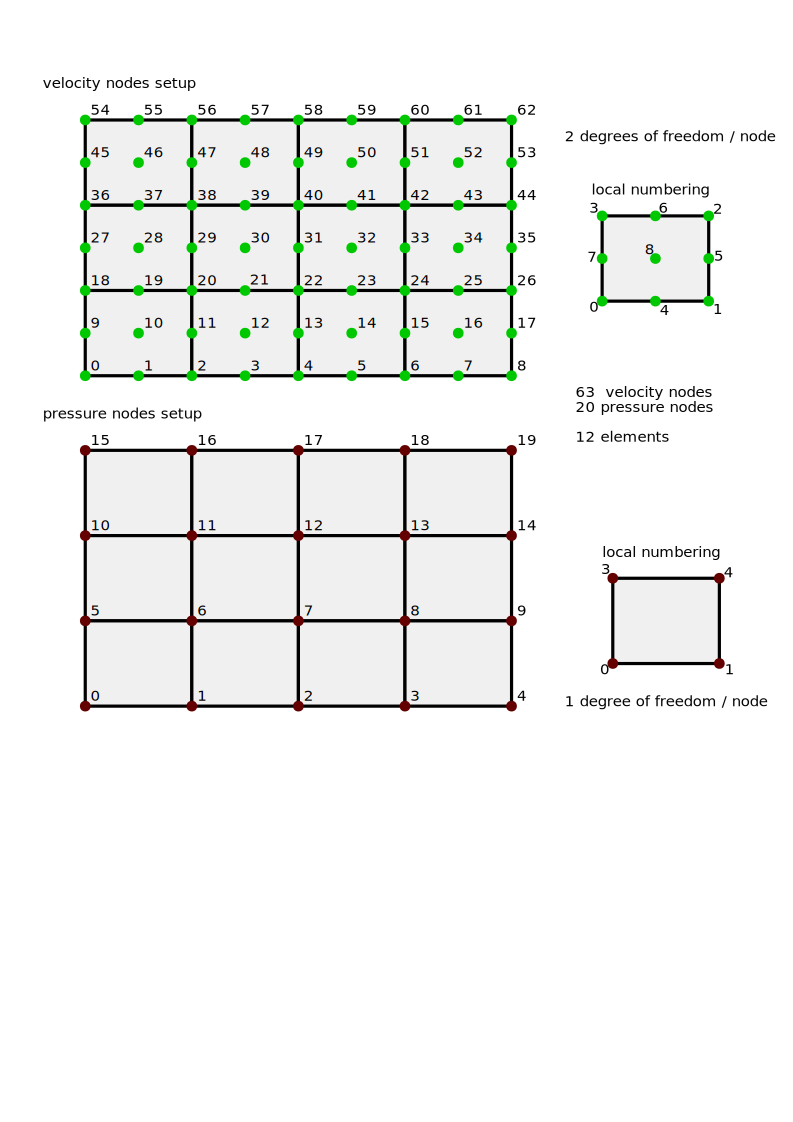
\includegraphics[width=10cm]{python_codes/fieldstone_18/images/q2q1setup}
\end{center}

\begin{center}
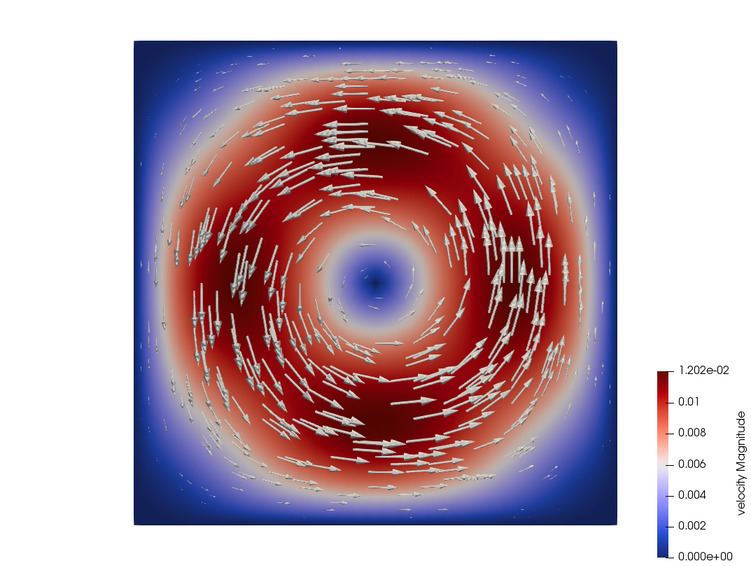
\includegraphics[width=7cm]{python_codes/fieldstone_18/results/mms/vel}
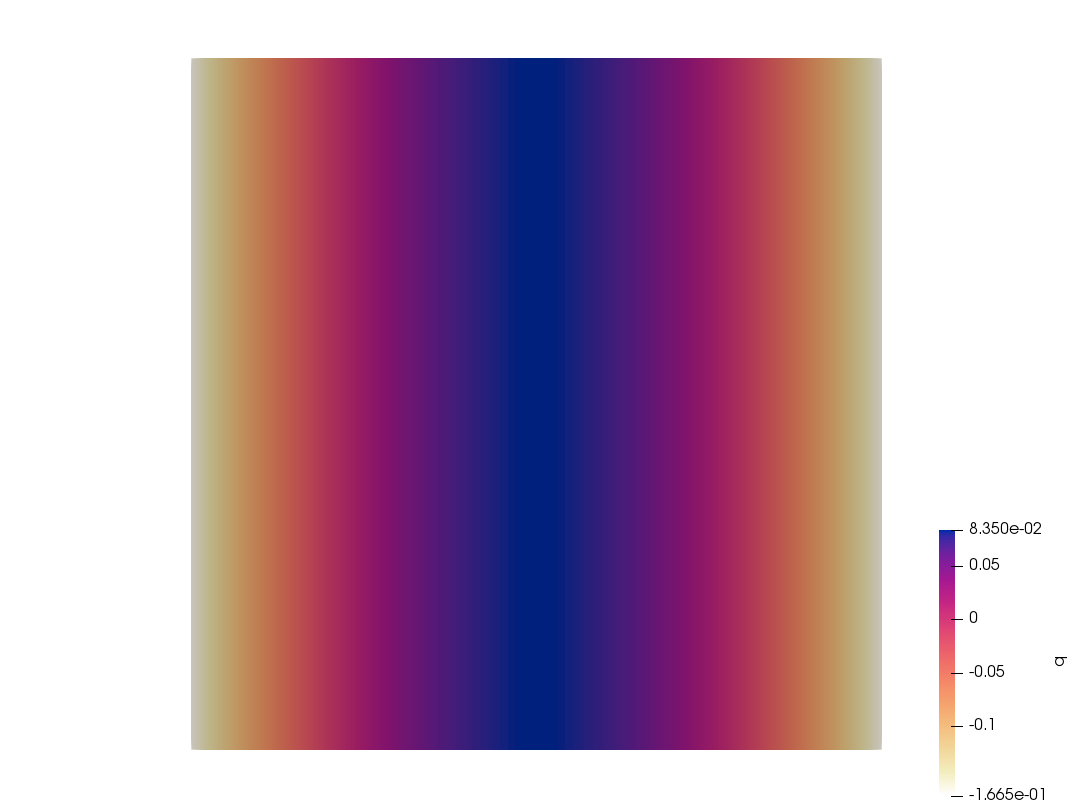
\includegraphics[width=7cm]{python_codes/fieldstone_18/results/mms/pressure}\\
{\captionfont velocity and pressure fields for $32\times 32$ elements grid}
\end{center}

\begin{center}
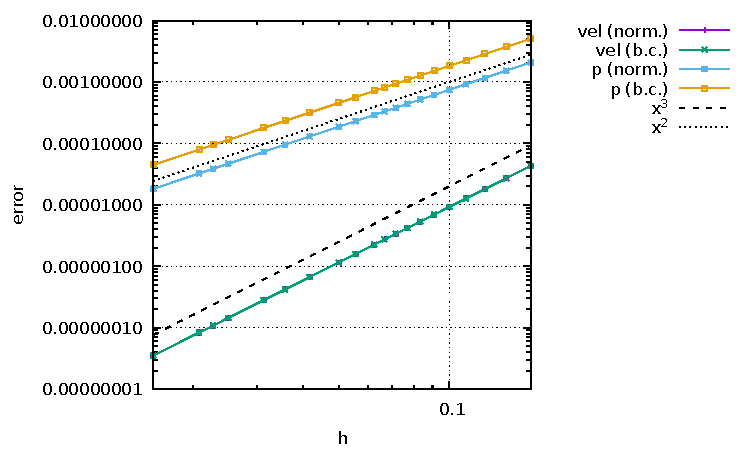
\includegraphics[width=12cm]{python_codes/fieldstone_18/results/mms/errors}\\
{\captionfont Velocity and pressure error convergence for both nullspace removal 
techniques. The zero average pressure approach yields smaller errors.}
\end{center}


%-----------------------------------------
\subsubsection*{Burman \& Hansbo manufactured solution}

The details of the numerical setup are presented in Section \ref{ss:mms_buha06}.

\begin{center}
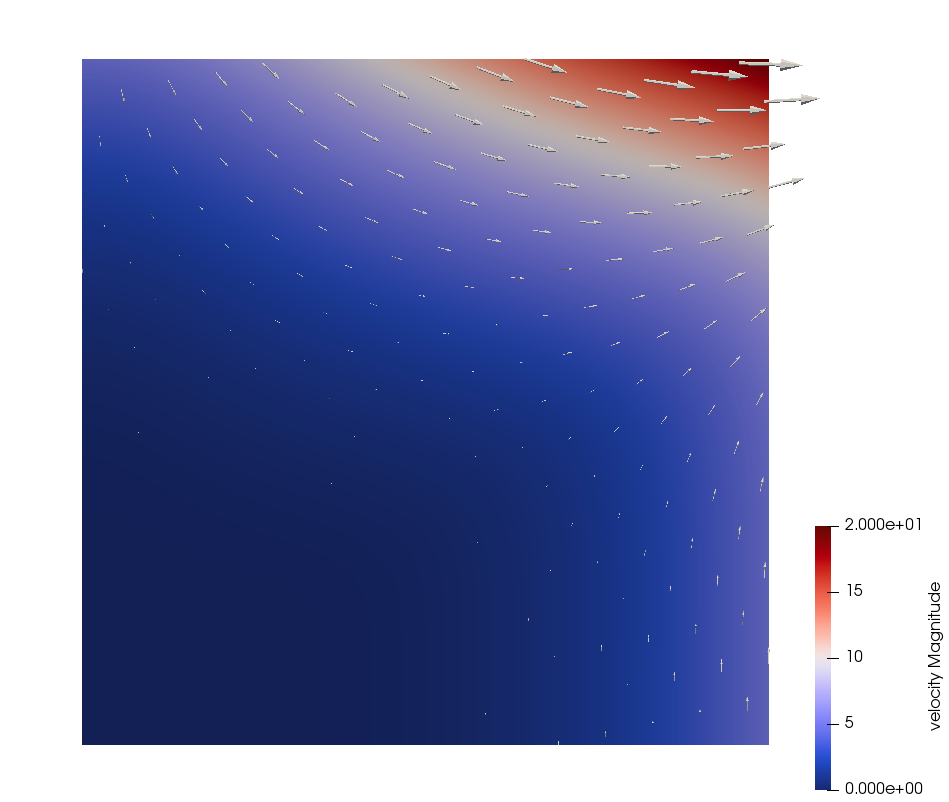
\includegraphics[width=5cm]{python_codes/fieldstone_18/results/buha06/vel}
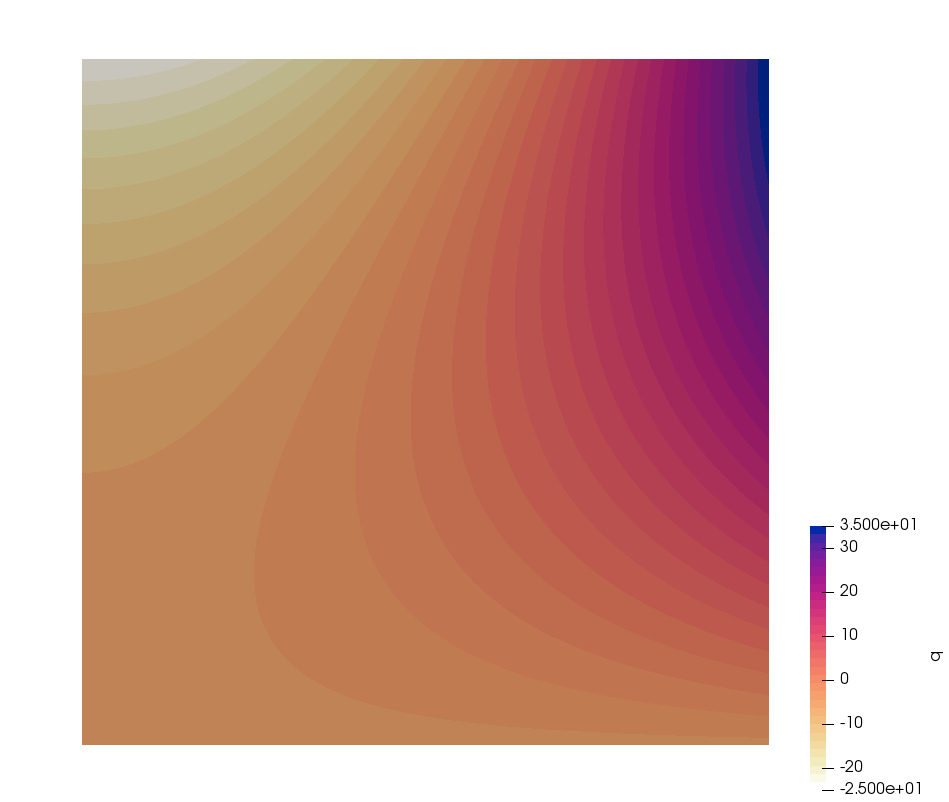
\includegraphics[width=5cm]{python_codes/fieldstone_18/results/buha06/p}\\
{\captionfont velocity and pressure fields for $64\times 64$ elements grid}
\end{center}

\begin{center}
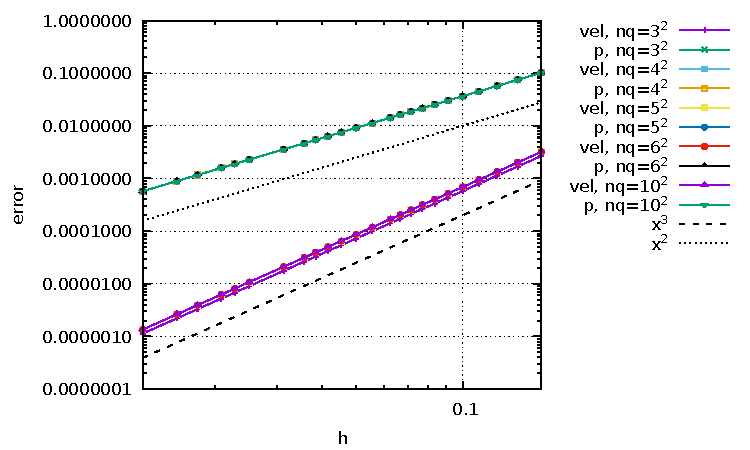
\includegraphics[width=12cm]{python_codes/fieldstone_18/results/buha06/errors}\\
{\captionfont Velocity and pressure error convergence. Zero average.}
\end{center}

No good reason to run such higher numbers of quadrature points.


%-----------------------------------------
\subsubsection*{Stokes sphere benchmark}

The setup is described in Section~\ref{ss:stokes_sphere2D}.

\begin{center}
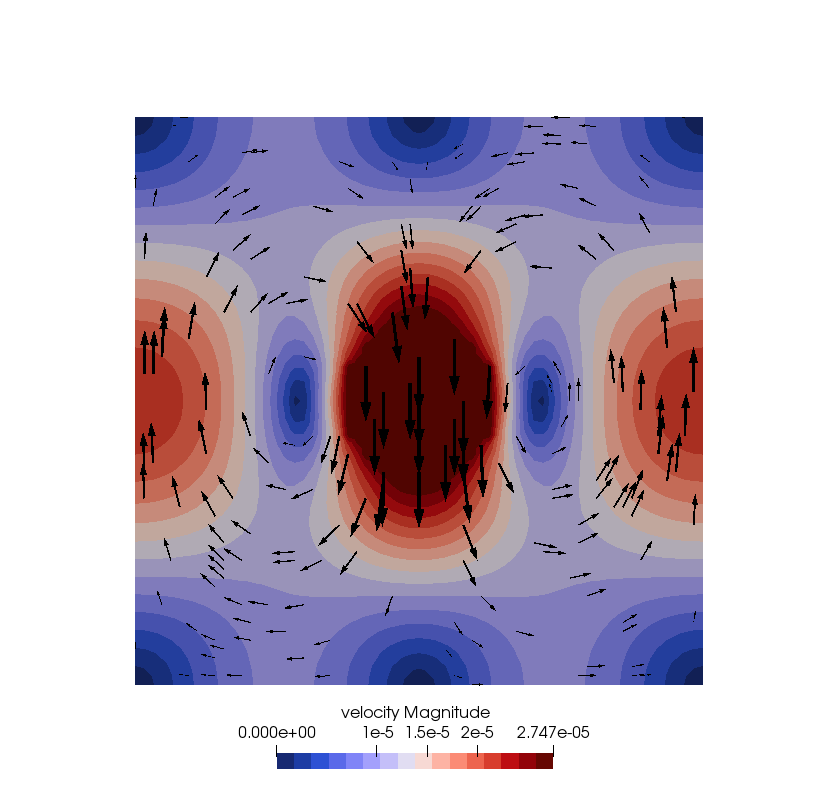
\includegraphics[width=7cm]{python_codes/fieldstone_18/results/sphere/vel}
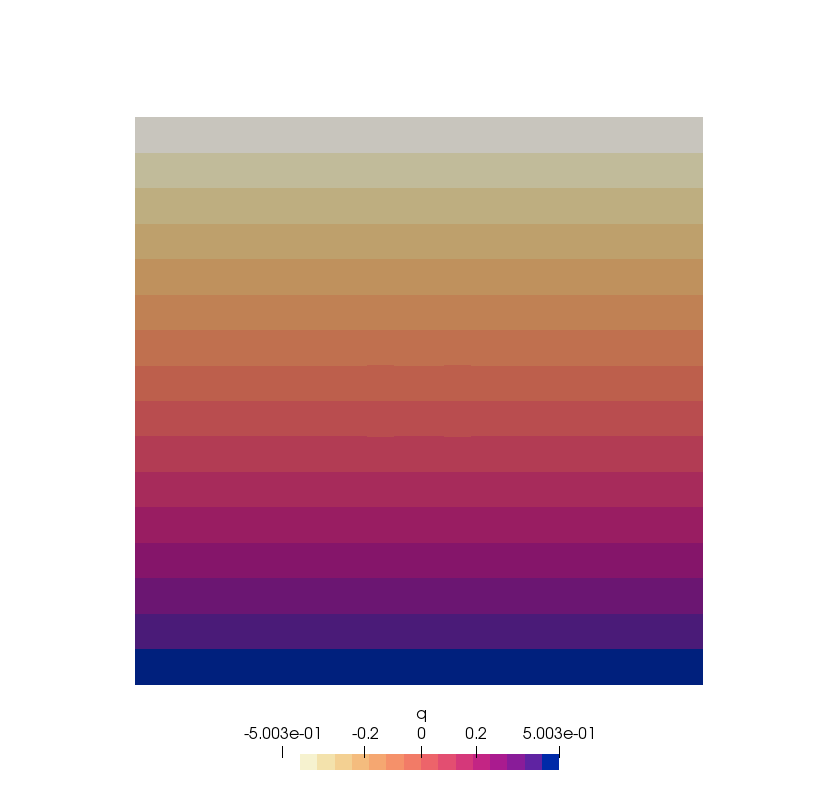
\includegraphics[width=7cm]{python_codes/fieldstone_18/results/sphere/press}\\
{\captionfont velocity and pressure fields for $32\times 32$ elements grid and $3^2$
quadrature points per element.}
\end{center}

%-----------------------------------------
\subsubsection*{Sinking block benchmark}

The setup is described in Section~\ref{ss:sinking_block}.

\paragraph{Free slip boundary conditions (FS)}

\begin{center}
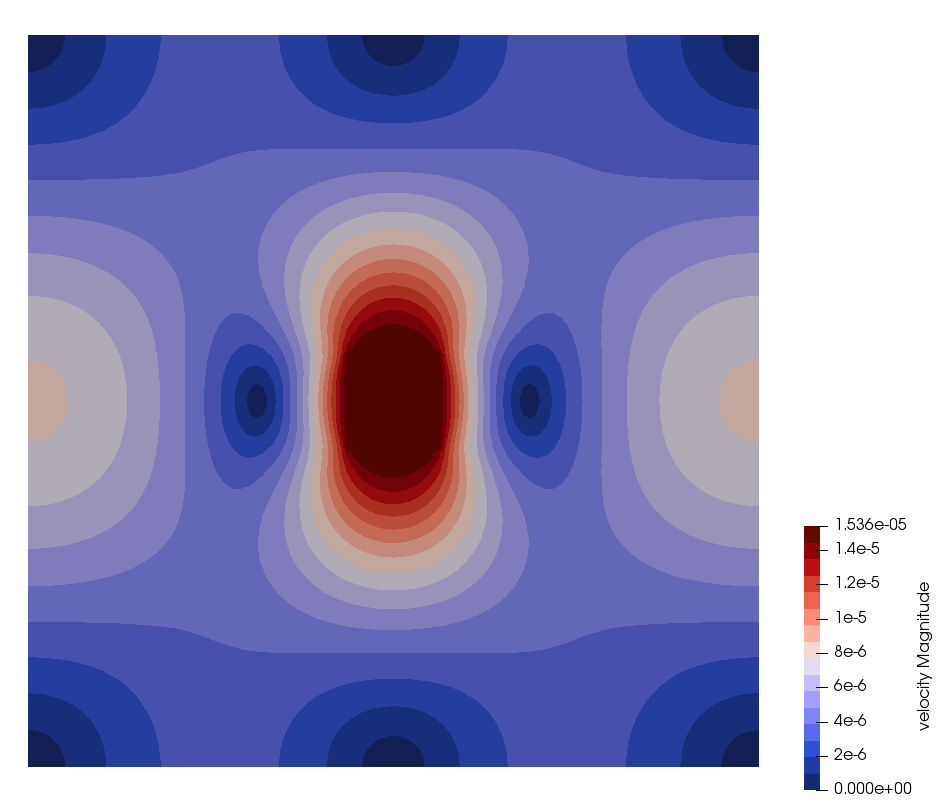
\includegraphics[width=7cm]{python_codes/fieldstone_18/results/block/FS/vel}
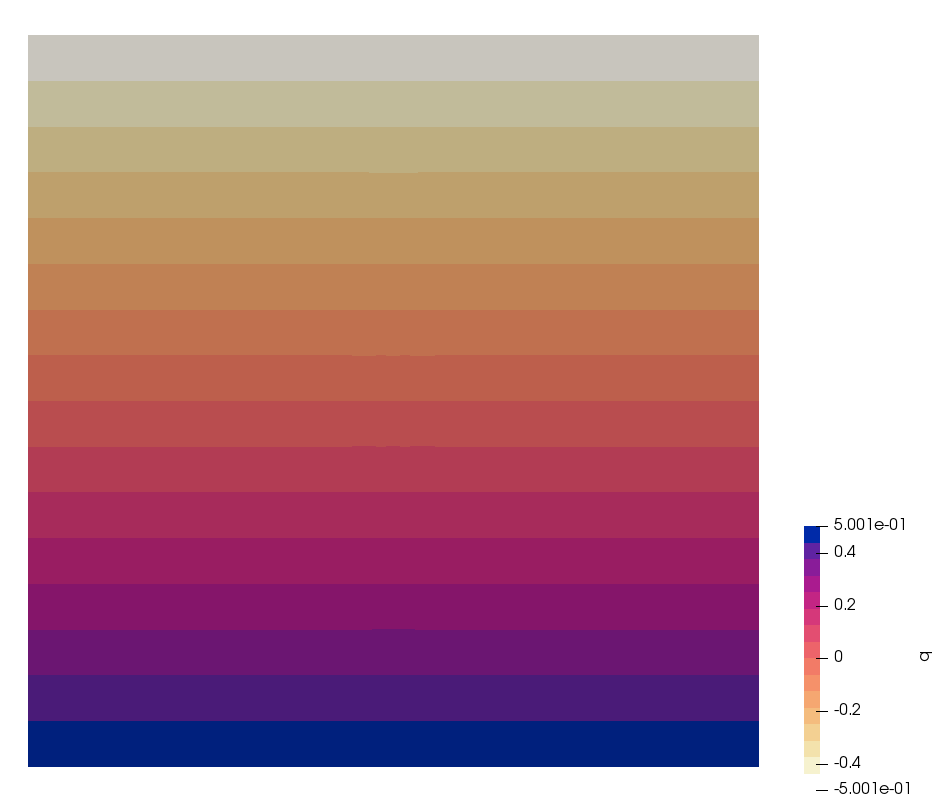
\includegraphics[width=7cm]{python_codes/fieldstone_18/results/block/FS/press}\\
{\captionfont velocity and pressure fields for $48\times 48$ elements grid and $3^2$
quadrature points per element.}
\end{center}


\begin{center}
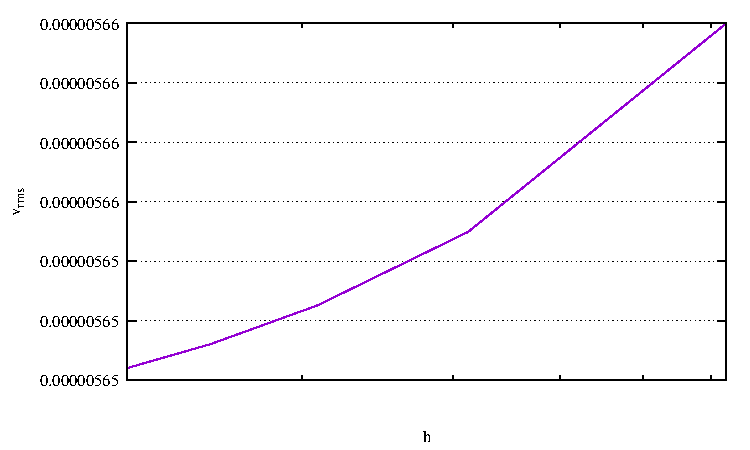
\includegraphics[width=5.7cm]{python_codes/fieldstone_18/results/block/vrms}
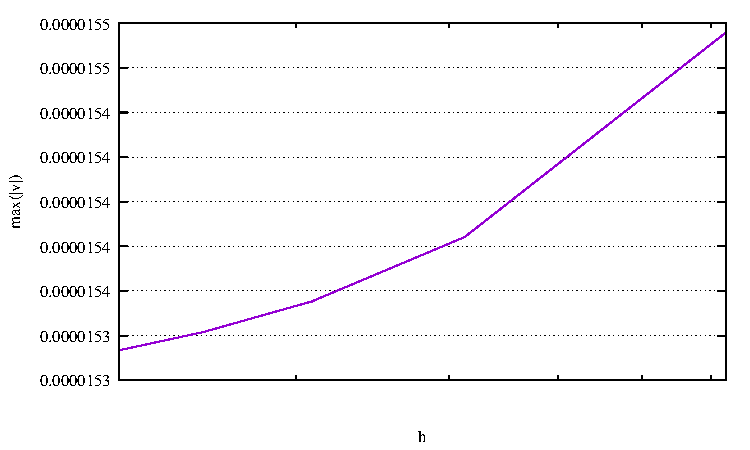
\includegraphics[width=5.7cm]{python_codes/fieldstone_18/results/block/max_vel}\\
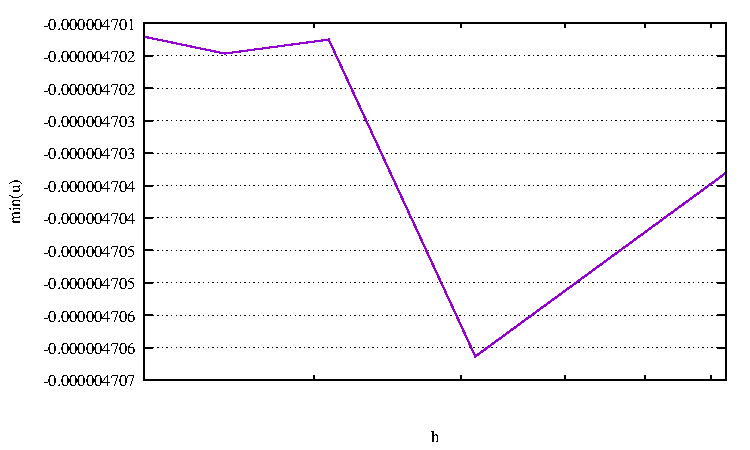
\includegraphics[width=5.7cm]{python_codes/fieldstone_18/results/block/min_u}
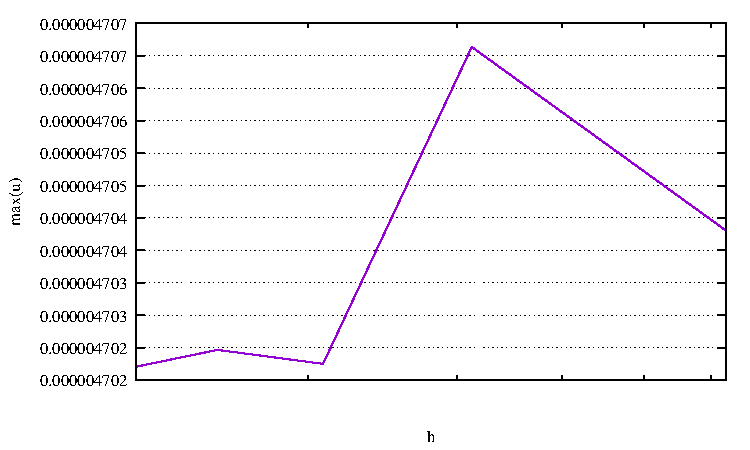
\includegraphics[width=5.7cm]{python_codes/fieldstone_18/results/block/max_u}\\
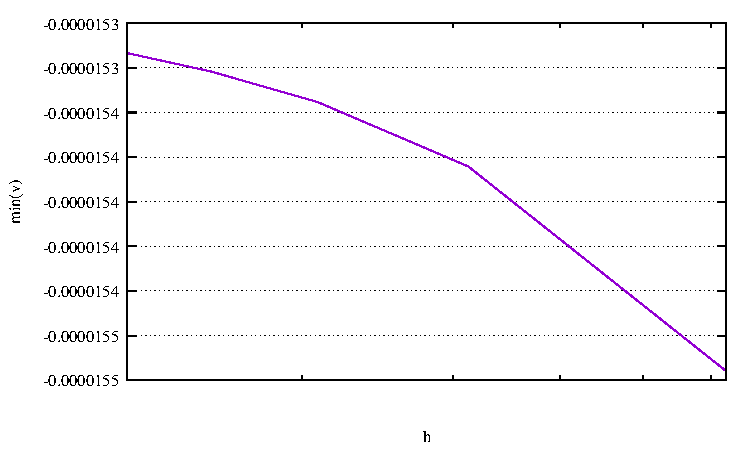
\includegraphics[width=5.7cm]{python_codes/fieldstone_18/results/block/min_v}
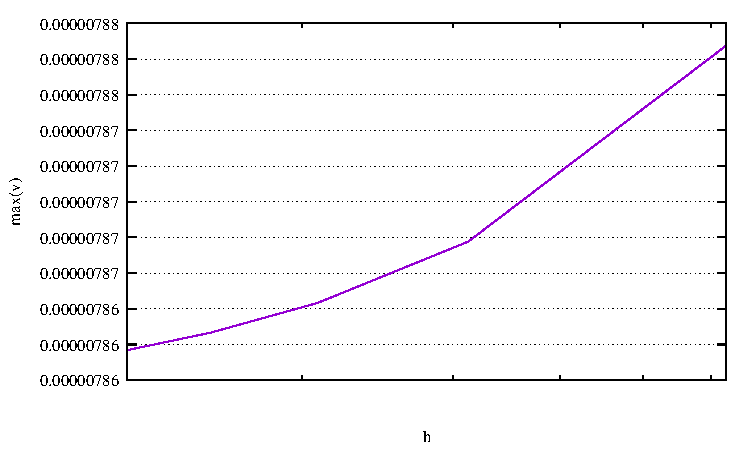
\includegraphics[width=5.7cm]{python_codes/fieldstone_18/results/block/max_v}\\
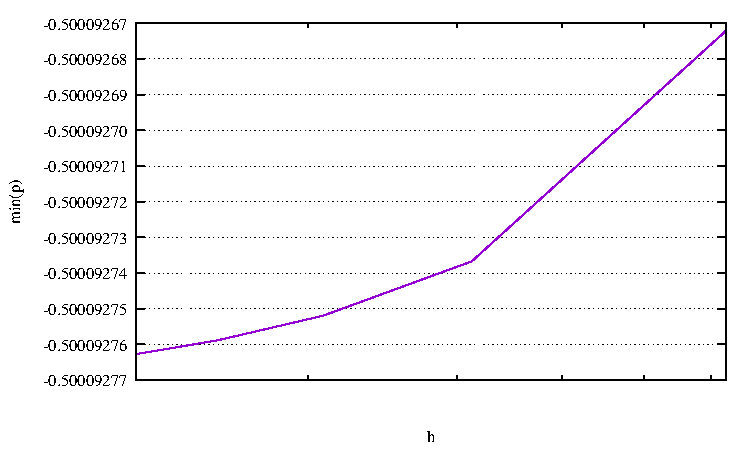
\includegraphics[width=5.7cm]{python_codes/fieldstone_18/results/block/min_p}
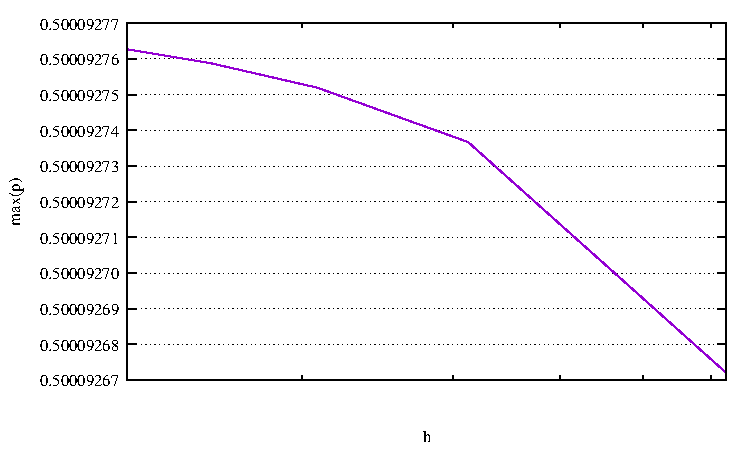
\includegraphics[width=5.7cm]{python_codes/fieldstone_18/results/block/max_p}\\
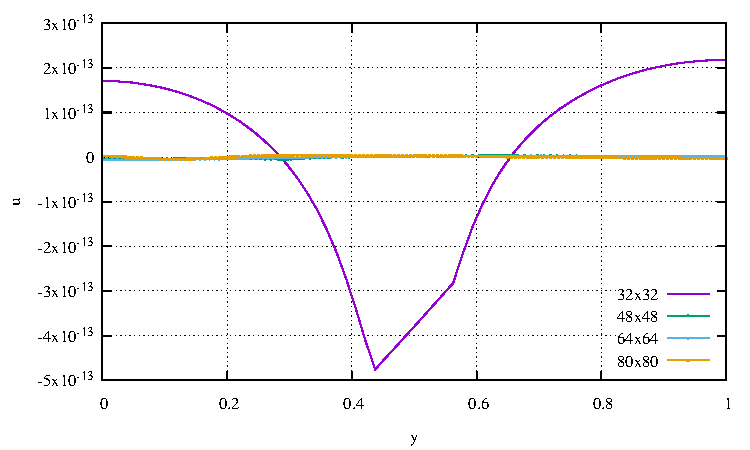
\includegraphics[width=5.7cm]{python_codes/fieldstone_18/results/block/profile_u_FS}
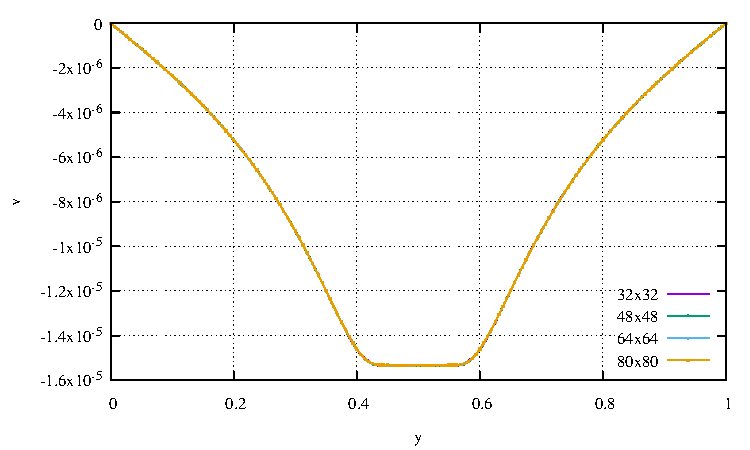
\includegraphics[width=5.7cm]{python_codes/fieldstone_18/results/block/profile_v_FS}
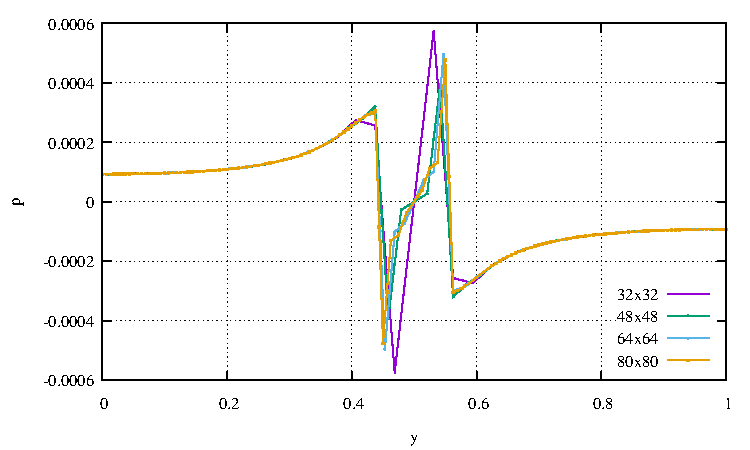
\includegraphics[width=5.7cm]{python_codes/fieldstone_18/results/block/profile_p_FS}
\end{center}

\paragraph{No slip boundary conditions (NS)}



\begin{center}
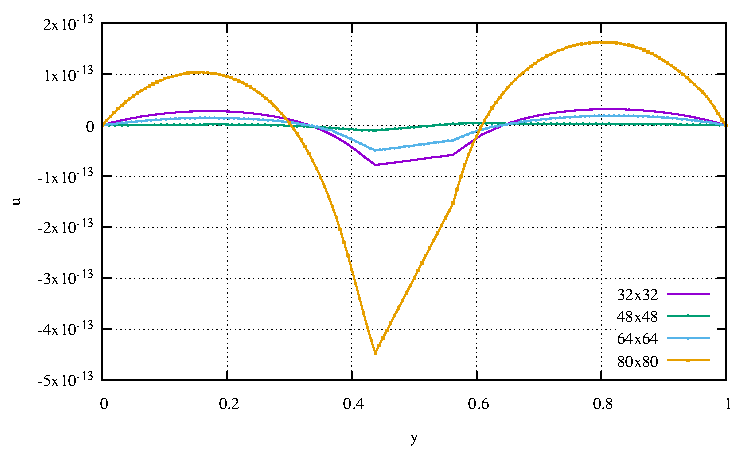
\includegraphics[width=5.7cm]{python_codes/fieldstone_18/results/block/profile_u_NS}
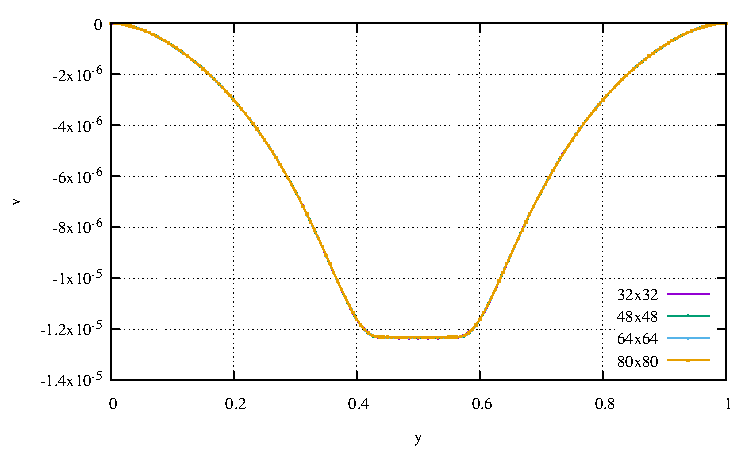
\includegraphics[width=5.7cm]{python_codes/fieldstone_18/results/block/profile_v_NS}
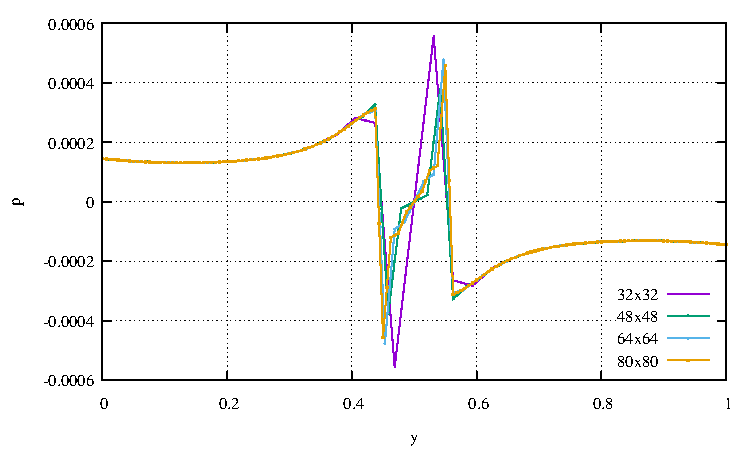
\includegraphics[width=5.7cm]{python_codes/fieldstone_18/results/block/profile_p_NS}
\end{center}



